%%%%%%%%%%%%%%%%%%%%%%%%%%%%%%%%%%%%%%%%%%%%%%%%%%%%%%%%%%%%%%%%%%
%%%%%%%% ICML 2016 EXAMPLE LATEX SUBMISSION FILE %%%%%%%%%%%%%%%%%
%%%%%%%%%%%%%%%%%%%%%%%%%%%%%%%%%%%%%%%%%%%%%%%%%%%%%%%%%%%%%%%%%%

% Use the following line _only_ if you're still using LaTeX 2.09.
%\documentstyle[icml2016,epsf,natbib]{article}
% If you rely on Latex2e packages, like most moden people use this:
\documentclass{article}

% use Times
\usepackage{times}
% For figures
\usepackage{graphicx} % more modern
%\usepackage{epsfig} % less modern
\usepackage{subfigure} 

% For citations
\usepackage{natbib}

% For algorithms
\usepackage{algorithm}
\usepackage{algorithmic}
\usepackage{psfrag,graphicx,graphics,epstopdf,colortbl}
\usepackage{fancyhdr}
\usepackage{amsmath,amsfonts}
\usepackage{amsthm,amssymb,amsopn}
\usepackage{wrapfig}


% As of 2011, we use the hyperref package to produce hyperlinks in the
% resulting PDF.  If this breaks your system, please commend out the
% following usepackage line and replace \usepackage{icml2016} with
% \usepackage[nohyperref]{icml2016} above.
\usepackage{hyperref}

% Packages hyperref and algorithmic misbehave sometimes.  We can fix
% this with the following command.
\newcommand{\theHalgorithm}{\arabic{algorithm}}

% Employ the following version of the ``usepackage'' statement for
% submitting the draft version of the paper for review.  This will set
% the note in the first column to ``Under review.  Do not distribute.''
\usepackage{icml2016} 

% Employ this version of the ``usepackage'' statement after the paper has
% been accepted, when creating the final version.  This will set the
% note in the first column to ``Proceedings of the...''
%\usepackage[accepted]{icml2016}


% The \icmltitle you define below is probably too long as a header.
% Therefore, a short form for the running title is supplied here:
\icmltitlerunning{Counterfactual Fairness}

\begin{document} 

\twocolumn[
\icmltitle{Counterfactual Fairness}

% It is OKAY to include author information, even for blind
% submissions: the style file will automatically remove it for you
% unless you've provided the [accepted] option to the icml2016
% package.
\icmlauthor{Your Name}{email@yourdomain.edu}
\icmladdress{Your Fantastic Institute,
            314159 Pi St., Palo Alto, CA 94306 USA}
\icmlauthor{Your CoAuthor's Name}{email@coauthordomain.edu}
\icmladdress{Their Fantastic Institute,
            27182 Exp St., Toronto, ON M6H 2T1 CANADA}

% You may provide any keywords that you 
% find helpful for describing your paper; these are used to populate 
% the "keywords" metadata in the PDF but will not be shown in the document
\icmlkeywords{causality, fairness}

\vskip 0.3in
]




\begin{abstract}
There has been immense recent interest in fairness in machine learning. Algorithms trained on data from the real world, which for historical reasons may produce unfair outcomes, will tend to perpetuate that unfairness through their predictions. For example, racial disparities in the US criminal justice system (cite) may be perpetuated through the predictions of recidivism risk assessment algorithms (cite). A number of recent papers have attempted to address this issue by defining various notions of fairness and proposing algorithms designed to give the best possible predictions while satisfying that definition of fairness. In this work, we leverage the language and methodology developed in the literature on causal inference to address fairness.
%For instance, imagine a bank wishes to train a machine learning model to predict whether or not an individual should be given a loan to buy a house. If the bank simply tries to learn a model that accurately predicts who to loan to solely based on whether the loan will be paid back. 
%Specifically, we would want any model that offers house loans to individuals to not be biased by an individual's race in granting such loans. Or we would like a
%with respect to race, gender, and any other individual attribute 
\end{abstract} 


\section{Introduction}
%!TEX root=ricardo_draft.tex
% ml is now everywhere
Machine learning is now used in fields as diverse as credit scoring (CITE), crime prediction (CITE), and loan assessment (CITE). As machine learning enters these new areas it is necessary for the modeler to think beyond the simple objective of maximizing prediction accuracy.

% in these new ml fields, we cannot discriminate
% discrimination can happen in multiple ways
% - direct discrimination
In particular, for many of these new applications, it is crucial to consider whether the predictions of a machine learning model are \emph{fair}. For instance, imagine a bank wishes to train a machine learning model to predict whether or not an individual should be given a loan to buy a house. The bank wishes to use historical lending data on whether or not a loan was paid back, along with personal information on individuals. If the bank simply tries to learn a model that accurately predicts who to loan to solely based on whether the loan will be paid back, it may unjustly favor giving loans to applicants of a particular demographic group, due to historical and present prejudices. The Obama Administration released a report that precisely describes this, and urged machine learning practicioners to analyze ``how technologies can deliberately or inadvertently perpetuate, exacerbate, or mask discrimination"\footnote{https://obamawhitehouse.archives.gov/blog/2016/05/04/big-risks-big-opportunities-intersection-big-data-and-civil-rights}.

As a result, there has been immense interest recently in designing machine learning algorithms that make fair predictions. (CITE A MILLION PAPERS). In large part each work focuses on formalizing fairness into a concrete definition that can be tested, and for which algorithms can be developed. By defining fairness concretely, one can design specific algorithms to satisfy such definitions. 



%  This could be due to many factors that are observed and unobserved in the features of a given dataset such as:
% \begin{itemize}
% \item (\emph{observed}) race could be a feature in the dataset, thus any algorithm using this feature for prediction is directly using race to discriminate.
% \item (\emph{observed}) other features could be proxies for race, such as where an individual currently lives.
% \item (\emph{unobserved}) there may exist historical biases that make it more difficult for certain races to secure employment, thereby making a direct comparison between two individuals of different races unfair and could actually harm prediction (as a high-earning individual in one race may have had to work much harder to obtain work than a similar individual in another race, thus it may be crucial to look beyond observed features and favor the hard-working individual).
% \item (\emph{unobserved}) the historical bank data may favor giving loans to individuals of a certain race because of prejudiced lenders.
% \end{itemize}
% These are just a few possible sources of unfairness that an unaware classifier could exploit in order to make more accurate predictions.

% there's a lot of interest in this
% There has been immense interest recently in designing machine learning algorithms that make fair predictions. (CITE A MILLION PAPERS). In large part each work focuses on formalizing fairness into a concrete definition that can be tested, and for which algorithms can be developed. 

% By defining fairness concretely, one can design specific algorithms to satisfy such definitions. The hope is that such algorithms can begin to address the calls of various governing bodies about the need for fairness in automated algorithms. For instance, in the United States the Obama Administration has issued two reports (CITE), the first warning individuals about ``the potential of encoding discrimination in automated decisions" and the second describing ``how technologies can deliberately or inadvertently perpetuate, exacerbate, or mask discrimination"\footnote{https://obamawhitehouse.archives.gov/blog/2016/05/04/big-risks-big-opportunities-intersection-big-data-and-civil-rights}. Thus there is significant interest defining fairness in order to address it.

% a lot of this work just proposes a new definition of fairness and checks it
% these definitions may or may not be appropriate for a given problem
In large part, the initial work on fairness in machine learning has focused on formalizing the above definitions and using them to solve a discrimination problem in a certain dataset. Unfortunately, for a practitioner, law-maker, judge, or anyone else who is interested in implementing algorithms that control for discrimination, it can be difficult to decide which definition of fairness to choose for the task at hand. Indeed, we demonstrate that depending on the relationship between a sensitive attribute and the data certain definitions of fairness can actually \emph{increase discrimination}.

% we propose a way to model data that allows a practitioner to assess what definitions of fairness are right for the problem at hand, and algorithms to ensure fairness
% OR
% we propose a way to interpret fairness...
% a) relationship between fairness and causality
% b) use pearl's models
% c) having an explicit model allows us to test fairness with the assumptions laid bare
% tension: Pearl already talks about discrimination, so we aren't really inventing new models. Are we even new in using these models to talk about fairness? Maybe... Pearl talks about variables that we might want to compute counterfactuals for in order to see if discrimination is happening.  
% Our proposal is:
% - situate a sensitive variable in a graph (not new).
% - Look at old definitions and see if anything bad could happen (new). 
% - Then define counterfactual fairness (new). 
% - Modeling helps us see where the weaknesses are in our assumptions and definitions (maybe not new)
% We don't want to see if every definition is counterfactually fair because then we're like everyone else, saying our definition is best
% 

In this work, we describe how techniques from causal inference can be used to formalize questions of fair prediction. Specifically, we develop a technique to leverage the causal models of Pearl \cite{pearl2009causal} to model the relationship between the sensitive attribute and data. Our contributions are as follows:
\begin{enumerate}
    \item We model questions of fairness within a causal framework. This allows us to directly model \emph{how} unfairness affects the data at hand.
    \item We introduce \emph{counterfactual fairness}, which enforces that a distribution over possible predictions for an individual should remain unchanged, in a world where an individual's sensitive attribute was changed.
    \item We analyze how enforcing existing definitions of fairness for different data may or may not lead to fair predictions.
    \item We devise techniques learning predictors that are counterfactually fair.
\end{enumerate}
%We demonstrate that by explicitly representing fairness within a causal model it becomes easy to critique different definitions of fairness as well the prediction methods that aim to accomplish these notions of fairness.











% RETHINK SPIN, ALWAYS RETHINK


\section{Fairness in machine learning}

\subsection{Fairness}

TODO

\subsection{Causal Models and Counterfactuals}

We will follow the framework of \cite{pearl:00}, where a causal
model is a triple $(U, V, F)$ of sets such that
\begin{itemize}
\item $U$ is a set of {\bf background} variables\footnote{These are
  sometimes called {\bf exogeneous variables}, but the fact that members of $U$
  might depend on each other is not relevant to what follows.}, which are generated by factors
outside of our potential control;
\item $V$ is a set of {\bf endogenous} variables, where each member is determined by
  other variables in $U \cup V$;
\item $F$ is a set of functions $\{f_1, \dots, f_n\}$, one for each $V_i \in V$, such
that $V_i = f_i(pa_i, U_{pa_i})$, $pa_i \subseteq V \backslash
\{V_i\}$ and $U_{pa_i} \subseteq U$. Such equations are also known as
{\bf structural equations} \citep{bol:89}.
\end{itemize}

The notation ``$pa_i$'' is motivated by the extra assumption that the
model factorizes according to a directed acyclic graph (DAG). That is,
define a directed graph $\mathcal G$ where each node corresponds to an
element of $U \cup V$, and each edge $V_i \leftarrow X$ is added if
and only if $X \in pa_i \cup U_{pa_i}$. We assume $\mathcal G$ is
acyclic.

The model is causal in the sense that, for a given probability model
$p(U)$ for the background variables, it entails the distribution of a
subset of $V$ given an {\bf intervention} in another subset of $V$.
The operational meaning of an intervention on $V_i$ at value $v$ is
the substitution of the equation $V_i = f_i(pa_i, U_{pa_i})$ with the
equation $V_i = v$. This captures the idea of an agent modifying a
system while being external to it. For instance, this can happen as a
randomized controlled trial that overrides the value of $V_i$ with a
treatment that sets it at $v$, a value chosen at random independently
of any other causes of the system. Pearl's do-calculus
\citep{pearl:00} provides a way of identifying features of 
interventional distributions, when possible, using only (estimates of) the joint
distribution of $V$ and the causal DAG.

Compared to independence constraints given by a DAG, the full
specification of $F$ requires much stronger assumptions but also leads
to much more specific claims. In particular, it allows for the
calculation of {\bf counterfactual} quantities. Without going into a
detailed coverage of the topic, consider the following counterfactual
statement, ``the value of $Y$ had $X$ been $x$'', for two endogenous
variables $X$ and $Y$ in a causal model. By assumption, the state of
any endogenous variable is fully determined by
the background variables and structural equations. The counterfactual is
modeled as the solution for $Y$ for a given $U = u$ where the equation(s)
for $X$ is (are) replaced with $X = x$.  We denote it by $Y_{X \leftarrow x}(u)$
\cite{pearl:00}.

Counterfactual inference, as specified by a causal model $(U, V, F)$,
is the computation of probabilities $P(Y_{X \leftarrow x}(U)\ |\ W =
w)$, where $W$, $X$ and $Y$ are subsets of $V$. Inference proceeds in
three steps, as explained in more detail in Chapter 4 of
\cite{pearl:16}:
\begin{enumerate}
\item For a given prior on $U$, compute the posterior distribution of $U$ given the evidence $W = w$;
\item Substitute the equations for $X$ with the interventional values $x$, resulting
     in the modified set of equations $F_x$;
\item Compute the implied distribution on the remaining elements of $V$
     using $F_x$ and the posterior $P(U\ | W = w)$.
\end{enumerate}

\section{The counterfactual approach}












\begin{figure*}[th!]
\begin{center}
\vspace{-2ex}
\centerline{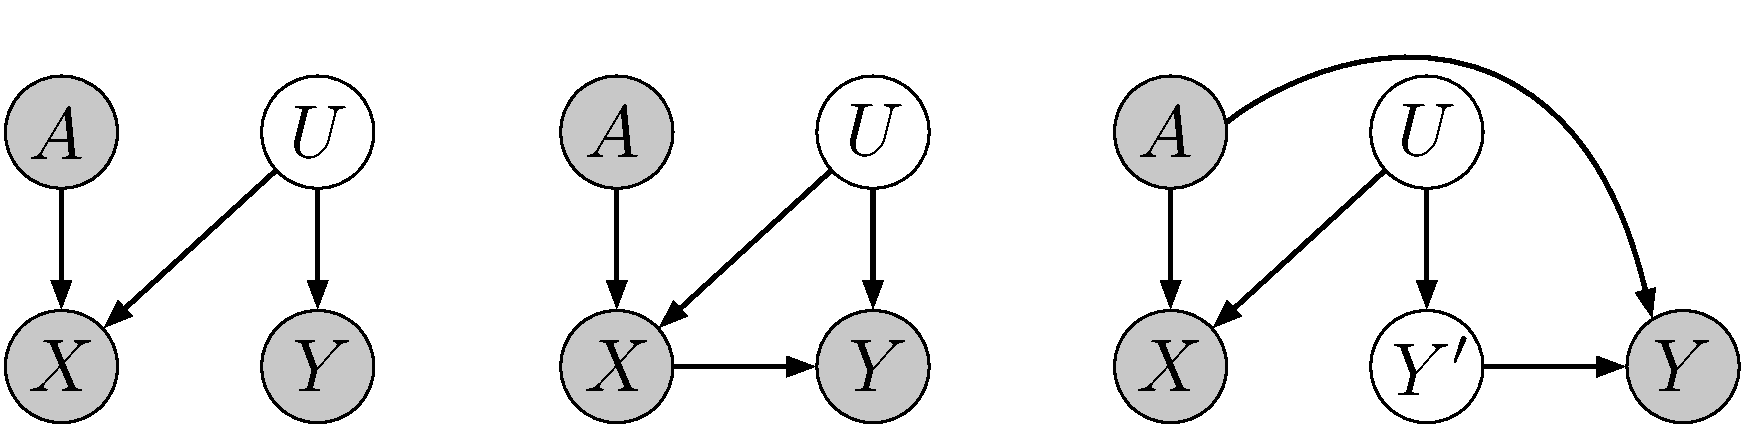
\includegraphics[width=\textwidth]{simple_models_no_q}}
\vspace{-2ex}
\caption{Three possible states of the world.\label{figure.simple_models}}
\vspace{-2ex}
\end{center}
\end{figure*}


\section{Unprejudicial Inference under Causal Structures}
\label{sec-1}

Much as we talk about variables being causally independent of one
another, it's possible to talk of predictions being counter factually
fair.

We say that a predictor of $Y$, $\hat Y(X,A)$ is causally
independent of $A$ if 
%
\[ \hat Y(X,A)=\hat Y(X,A)|\text{do}(A=a) \] 
%
In the general case, a classifier $\hat Y (X)$ that does not directly
depend on $A$ need not be causally independent of $A$ if $X$ depends on $A$.

We are interested in three related questions, illustrated by the
causal diagrams in figure 1. From left to right:

\begin{enumerate}
\item Given a $Y$ causally independent of $A$, can we learn a $\hat Y$,
causally independent of $A$ that accurately predicts $Y$?
\item Given a $Y$ causally \textbf{dependent} on $A$, can we learn a $\hat Y$,
causally independent of $A$ that predicts $Y$ as closely as possible?
\item Given a $Y'$, causally independent of $A$ but unobserved, and an
observed $Y$ which represents $Y$ corrupted by a function of $A$,
can we recover $Y'$?
\end{enumerate}

To simplify this problem, we first consider the linear case in where
variables are distributed Gaussianly and the dependencies are
additive, and related this to previous existing work on orthogonality
in fairness, before considering the more general case.

\subsection{Fair Learning in a Fair World}
\label{sec-1-1}
\subsection{Fair Learning in an Unfair World}
\label{sec-1-2}
\subsection{Recovering Fairness from Corrupted Data}
\label{sec-1-3}


\bibliography{bibliography}
\bibliographystyle{icml2016}

\end{document} 